\section{INTERCEPT TIMELINES}

\subsection{TERMINOLOGY}

\begin{tcoloritemize}
    \blueitem[Contact]
    \blueitem[Group]
    \blueitem[Picture]
\end{tcoloritemize}

\subsection[AR FLOW]{ACTIVE-RADAR MISSILE FLOW}

\begin{tcoloritemize}
    \blueitem[Launch-and-Leave]
    \blueitem[Launch-and-Decide]
\end{tcoloritemize}


\subsection{RANGE DEFINITIONS}

\begin{tcoloritemize}
    \blueitem[WEZ]
    \blueitem[MAR] \textbf{M}inimum \textbf{A}bort \textbf{R}ange

    \medskip
    minimum range at which fighter can perform an abort maneuver to kinematically defeat any launched bandit weapons 

    \blueitem[MSR] \textbf{M}inimum \textbf{S}hot \textbf{R}ange

    \medskip
    minimum range at which AIM-120 will go active before fighter reaches MAR if launched

    \blueitem[DOR] \textbf{D}esired \textbf{O}ut \textbf{R}ange
    \blueitem[TR] \textbf{T}ransition \textbf{R}ange
    \blueitem[MTR] \textbf{M}inimum \textbf{T}argeting \textbf{R}ange
    \blueitem[MRR] \textbf{M}inimum \textbf{R}ecommit \textbf{R}ange
    \blueitem[DR] \textbf{D}ecision \textbf{R}ange
\end{tcoloritemize}

\marginfigeometry

\subsection{SKATE TIMELINE}

\begin{checklistenumerate}[start=0]
    \blueitem[Pre-commit] maintain SA
    
    \begin{itemize}
        \item \textbf{Comms} --- monitor AWACS
        \item \textbf{Sensors} --- sanitize airspace
    \end{itemize}

    \blueitem[Commit]%
    \label{subsec:ttpaa:timeline:skate:commit}
    \marginpar{
        \captionsetup{type=figure}
        \centering
        \begin{tikzpicture}[figstyle]

            % coordinates
            \coordinate (fighter_start) at (0,0);
            \coordinate (bandit) at (10,80);

            \coordinate (cr) at (0,5);
            \coordinate (mtr) at (0,10);
            \coordinate (sort) at (0,20);
            \coordinate (tr) at (0,30);
            \coordinate (dor) at (0,40);
            \coordinate (mrr) at (15,20);
            \coordinate (shoot2) at (5,50);
            \coordinate (mar) at (5,55);
            \coordinate (wez) at (0,65);
            \coordinate (fighter_end) at (20,50);

            % range lines
            \draw[thin]
                (25,0) -- (25,80);

            \path let \p1=(wez) in 
            node[font=\footnotesize,anchor=west] at (25,\y1) {WEZ};
            \path let \p1=(mar) in 
            node[font=\footnotesize,anchor=west] at (25,\y1) {MAR};
            \path let \p1=(dor) in 
            node[font=\footnotesize,anchor=west] at (25,\y1) {DOR};
            \path let \p1=(mrr) in 
            node[font=\footnotesize,anchor=west] at (25,\y1) {MRR};
            \path let \p1=(tr) in 
            node[font=\footnotesize,anchor=west] at (25,\y1) {TR};
            \path let \p1=(mtr) in 
            node[font=\footnotesize,anchor=west] at (25,\y1) {MTR};
            \path let \p1=(cr) in 
            node[font=\footnotesize,anchor=west] at (25,\y1) {CR};

            
            
            \draw[thin, dashed] let \p1=(wez) in  
                (25,\y1) -- ++(-30, 0);
            \draw[thin, dashed] let \p1=(mar) in  
                (25,\y1) -- ++(-20, 0);
            \draw[thin, dashed] let \p1=(dor) in  
                (25,\y1) -- ++(-25, 0);
            \draw[thin, dashed] let \p1=(tr) in  
                (25,\y1) -- ++(-25, 0);
            \draw[thin, dashed] let \p1=(mrr) in  
                (25,\y1) -- ++(-10, 0);
            \draw[thin, dashed] let \p1=(mtr) in  
                (25,\y1) -- ++(-25, 0);
            \draw[thin, dashed] let \p1=(cr) in  
                (25,\y1) -- ++(-25, 0);

            % bandit wez
            \draw[fill=red!40]
                (bandit)
                -- ++(-60:15)
                arc (-60:-120:15)
                -- (bandit);
            
            % timeline
            \draw[->] 
                (fighter_start) -- 
                node[below, pos=0]{
                    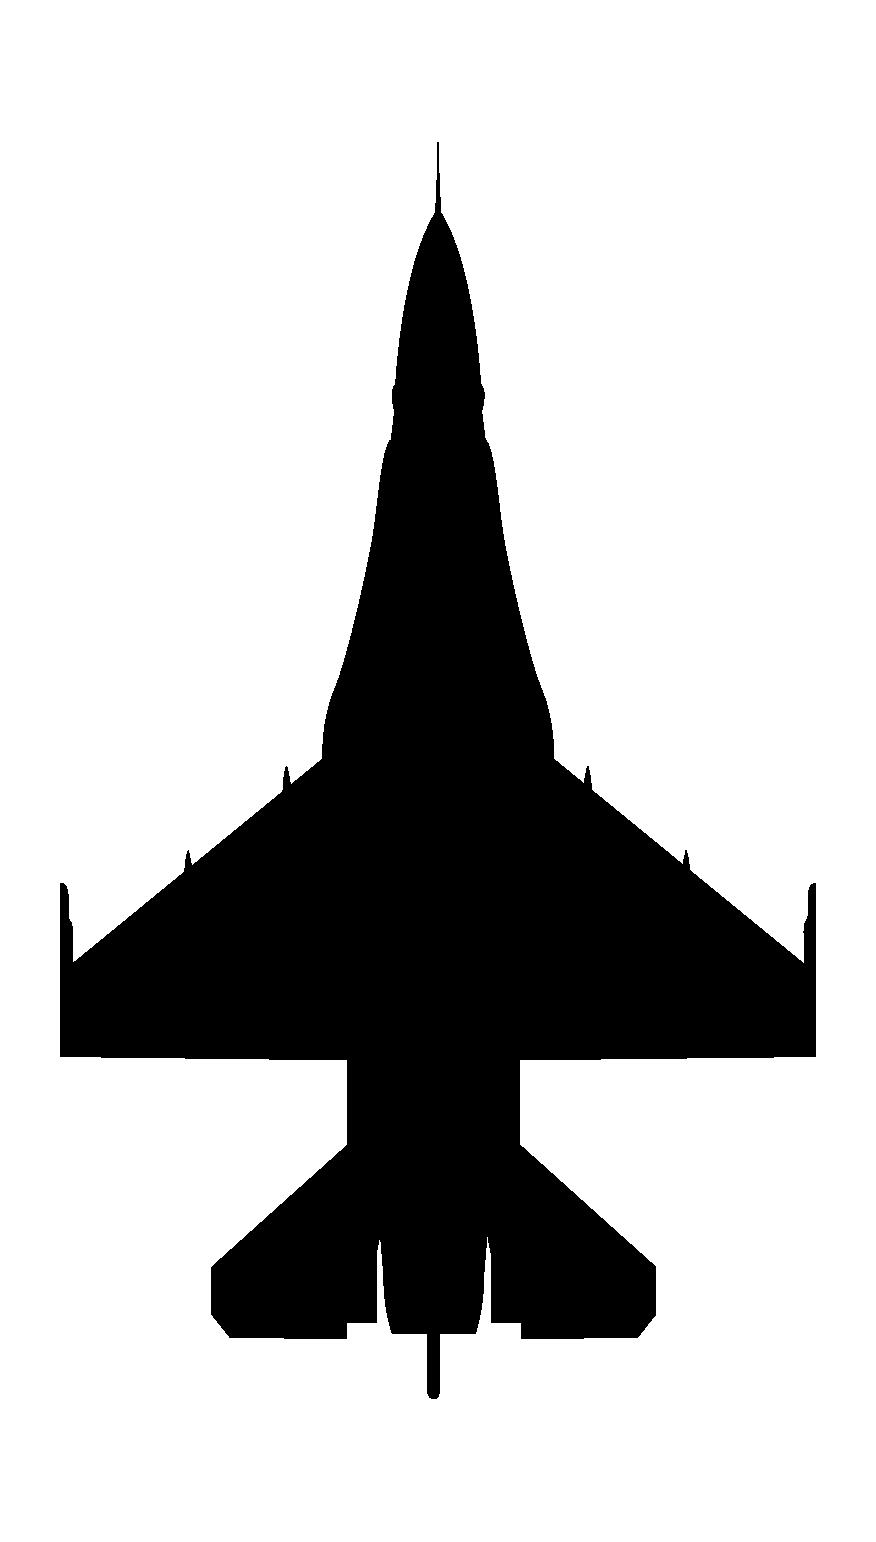
\includegraphics[
                    width=7.5mm,
                ]{diagrams/aircraft/silhouette_f16_top.pdf}} 
                (mtr);
            \draw[->]
                (mtr)
                -- (tr);
            \draw[->]
                (tr)
                -- (dor);
            \draw[->]
                (dor)
                arc (180:90:5) 
                -- ++(5,0)
                arc (90:0:5) 
                -- (mrr);
            \draw[->]
                (mrr)
                arc (0:-180:5) 
                -- (mar);
            \draw[->]
                (mar)
                arc (180:90:5) 
                -- ++(5,0)
                arc (90:0:5) 
                -- (fighter_end)
                node[below, pos=1, ]{
                    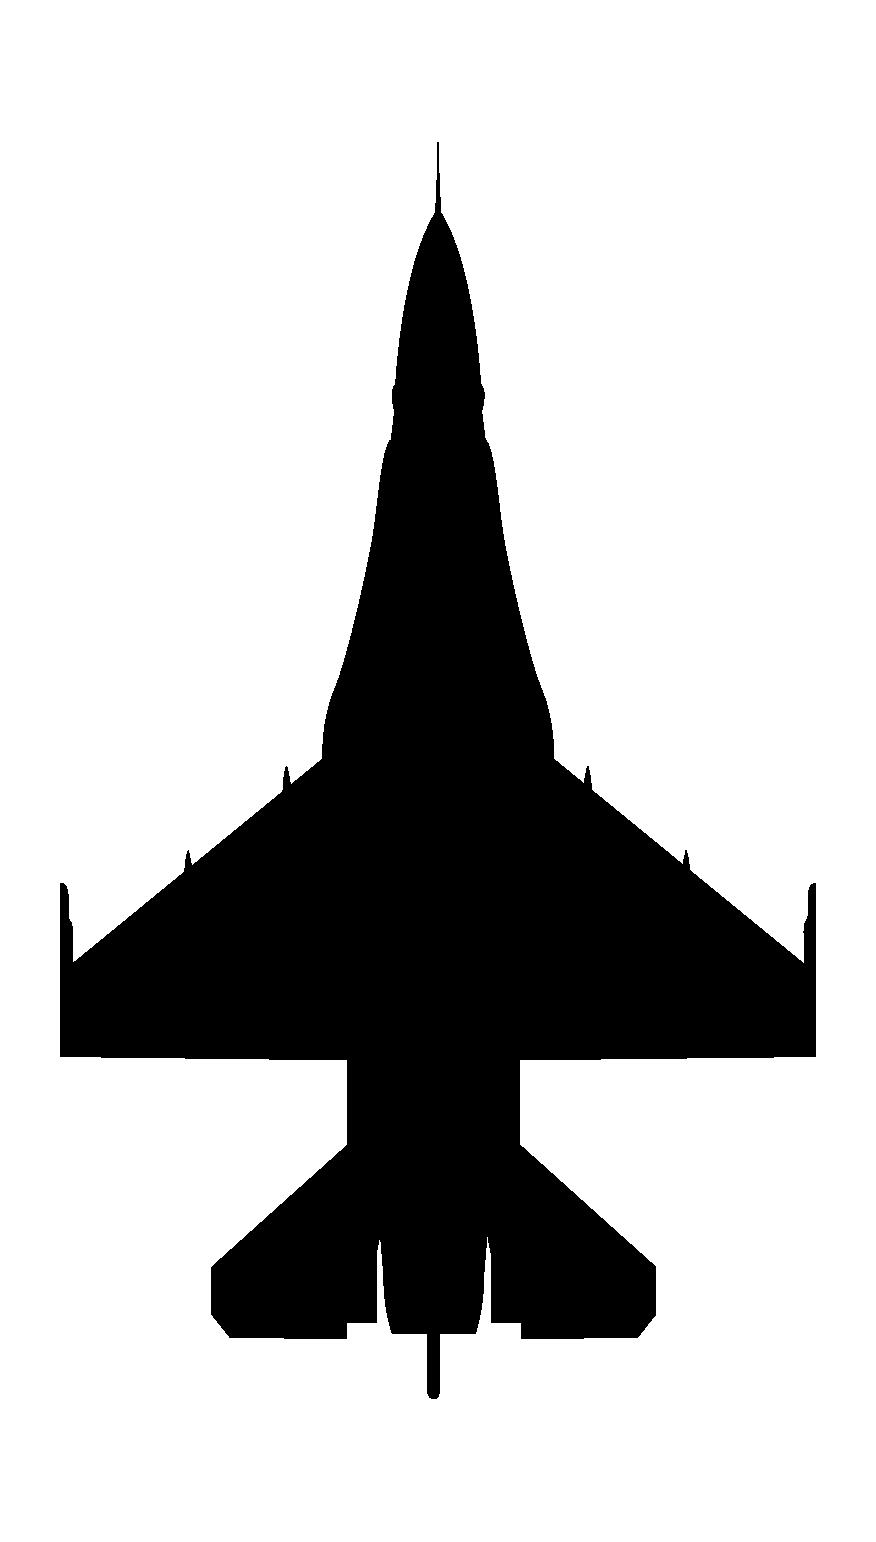
\includegraphics[
                        angle=180,
                        width=7.5mm,
                ]{diagrams/aircraft/silhouette_f16_top.pdf}};

            % bandit
            \node[] at (bandit) {
                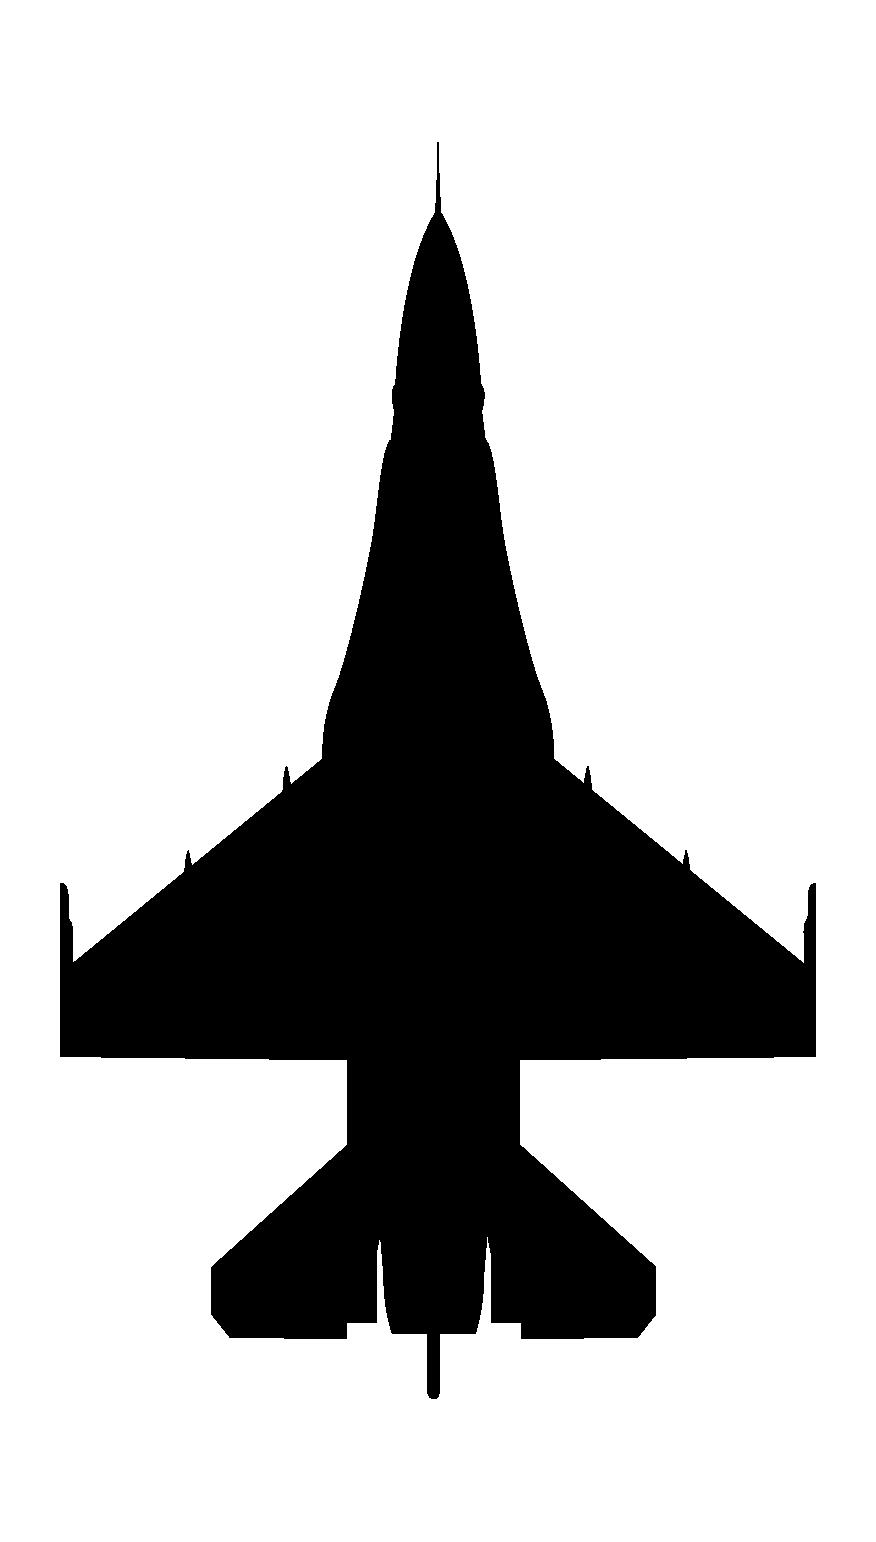
\includegraphics[
                    angle=180,
                    width=7.5mm,
            ]{diagrams/aircraft/silhouette_f16_top.pdf}};

            % labels
            \node[left, align=right, font=\small] at (cr) {
                \ref{subsec:ttpaa:timeline:skate:commit}
            };
            \node[left, align=right, font=\small] at (mtr) {
                \ref{subsec:ttpaa:timeline:skate:target}
            };
            \node[left, align=right, font=\small] at (sort) {
                \ref{subsec:ttpaa:timeline:skate:sort}
            };
            \node[left, align=right, font=\small] at (tr) {
                \ref{subsec:ttpaa:timeline:skate:shoot}
            };
            \node[left, align=right, font=\small] at (dor) {
                \ref{subsec:ttpaa:timeline:skate:out}
            };
            \node[left, align=right, font=\small] at (mrr) {
                \ref{subsec:ttpaa:timeline:skate:recommit}
            };
            \node[left, align=right, font=\small] at (shoot2) {
                \ref{subsec:ttpaa:timeline:skate:shoot2}
            };
            \node[left, align=right, font=\small] at (mar) {
                \ref{subsec:ttpaa:timeline:skate:out2}
            };

            % \filldraw[red] (tr) circle (2pt);
            % \filldraw[red] (mar) circle (2pt);

        \end{tikzpicture}
        \caption{Skate timeline}
        \label{fig:ttpaa:timeline:skate}
    }%
    \textbf{--- start of intercept timeline}
    \begin{itemize}
        \item AWACS picture or own FCR contacts meet briefed commit criteria
        \item flight leaves assigned patrol area
        \item \textbf{should be accomplished before CR}
    \end{itemize}

    \blueitem[Target]
    \label{subsec:ttpaa:timeline:skate:target}
    \begin{itemize}
        \item target call indicates responsibility to \\
        engage group in accordance with ROE
        \item flight members obtain radar contact
        \item \textbf{must be accomplished before MTR}
    \end{itemize}

    \blueitem[Sort]
    \label{subsec:ttpaa:timeline:skate:sort}
    \begin{itemize}
        \item flight members sort contacts
        \item flight members obtain FCR lock on assigned contact
    \end{itemize}

    \blueitem[Employment]
    \label{subsec:ttpaa:timeline:skate:shoot}
    \begin{itemize} 
        \item verify clear avenue of fire
        \item \textbf{DLZ} --- R\textsubscript{PI} to R\textsubscript{OPT}\\
        manual loft to maximize performance
        \item \textbf{crank post launch to minimize closure}
        \item \textbf{should be accomplished before TR}
    \end{itemize}

    \marnotebox{
        \small\textbf{\Cref{fig:ttpaa:timeline:skate} NOT to scale}
    }
    
    \marginpar{
        \captionsetup{type=figure}
        \centering
        \begin{tikzpicture}[figstyle]
            \node[boxedmarfigstyle] (fig) at (0,0) {
                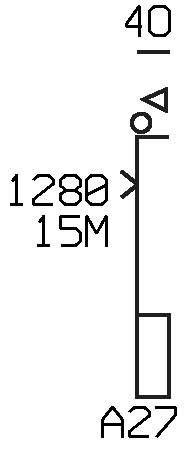
\includegraphics[
                    scale=0.5,
                ]{mfd/fcr_aa/aim120_subfig_dlz_prelaunch.pdf}
            };
        \end{tikzpicture}
        \caption{In-range DLZ}
    }

    \blueitem[Out]
    \label{subsec:ttpaa:timeline:skate:out}
    \begin{itemize}
        \item \textbf{before DOR, after pitbull}
        \item 5G slicing turn
    \end{itemize}
    \blueitem[Recommit] (if necessary)
    \label{subsec:ttpaa:timeline:skate:recommit}
    \begin{itemize}
        \item \textbf{range must be greater than MRR}
        \item fighter must reacquire \& sort bandit
    \end{itemize}
    \blueitem[Employment]
    \label{subsec:ttpaa:timeline:skate:shoot2}
    \begin{itemize}
        \item \textbf{must be accomplished before MAR}
    \end{itemize}
    \blueitem[Out]%
    \label{subsec:ttpaa:timeline:skate:out2}
    \textbf{--- 5G slicing turn at MAR}
\end{checklistenumerate}

\clearpage

\subsection{SHORT SKATE TIMELINE}
\subsection{BANZAI TIMELINE}

\marginpar{
    \captionsetup{type=figure}
    \centering
    \begin{tikzpicture}[figstyle]
        
        \draw[->] 
            (0,0) -- 
            node[below, pos=0]{
                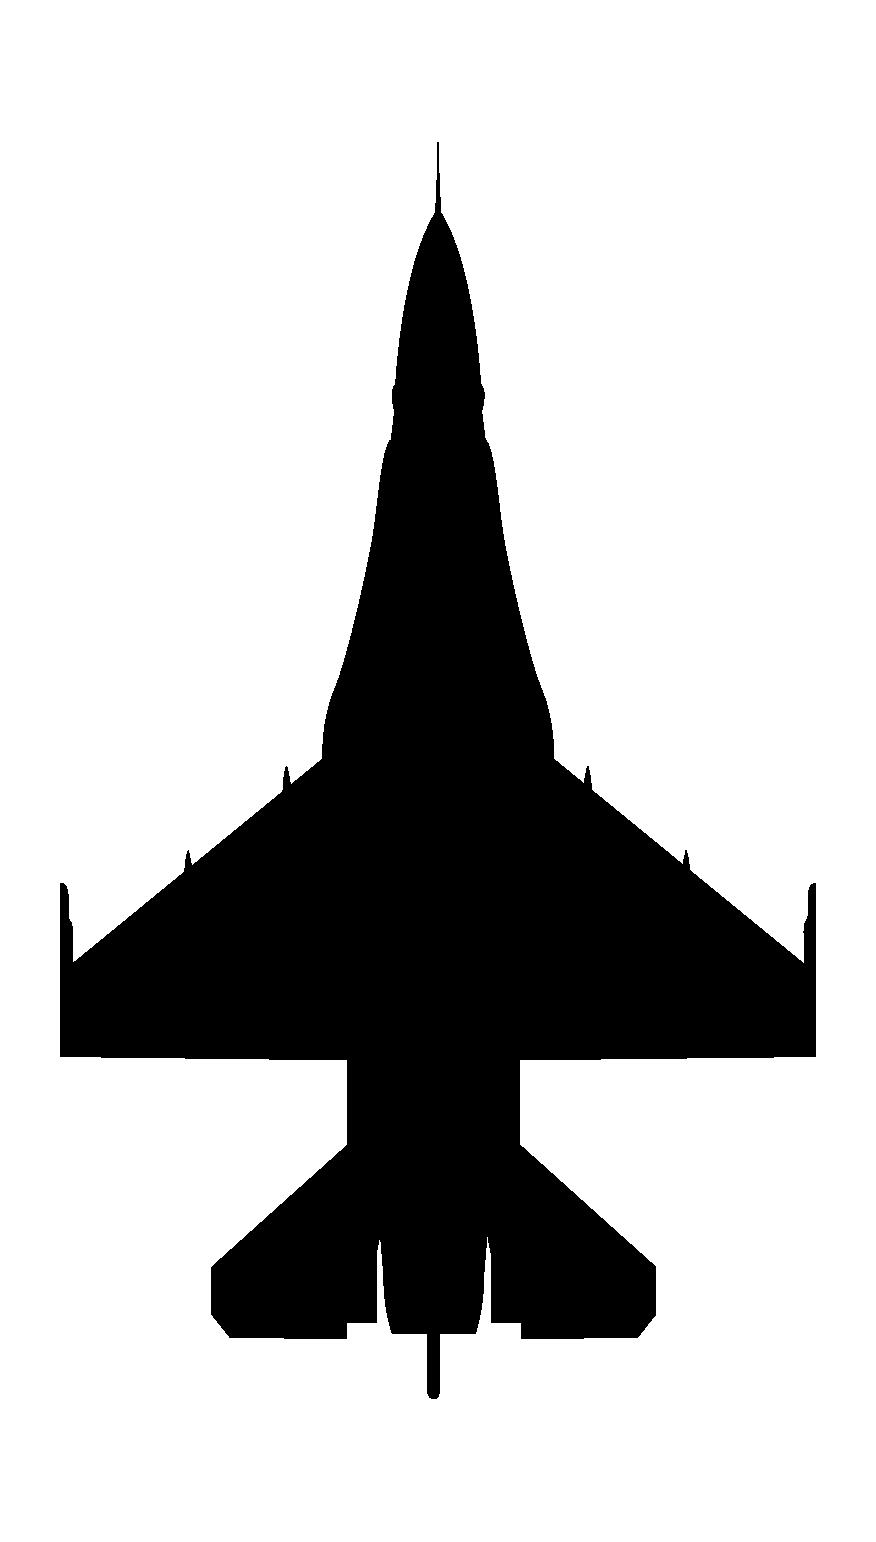
\includegraphics[
                width=7.5mm,
            ]{diagrams/aircraft/silhouette_f16_top.pdf}} 
            ++(0,20) 
            arc (180:90:5) 
            arc (-90:0:5) 
            -- ++(0,20) 
            arc (180:0:5) 
            -- ++(0,-50)
            node[below, pos=1, ]{
                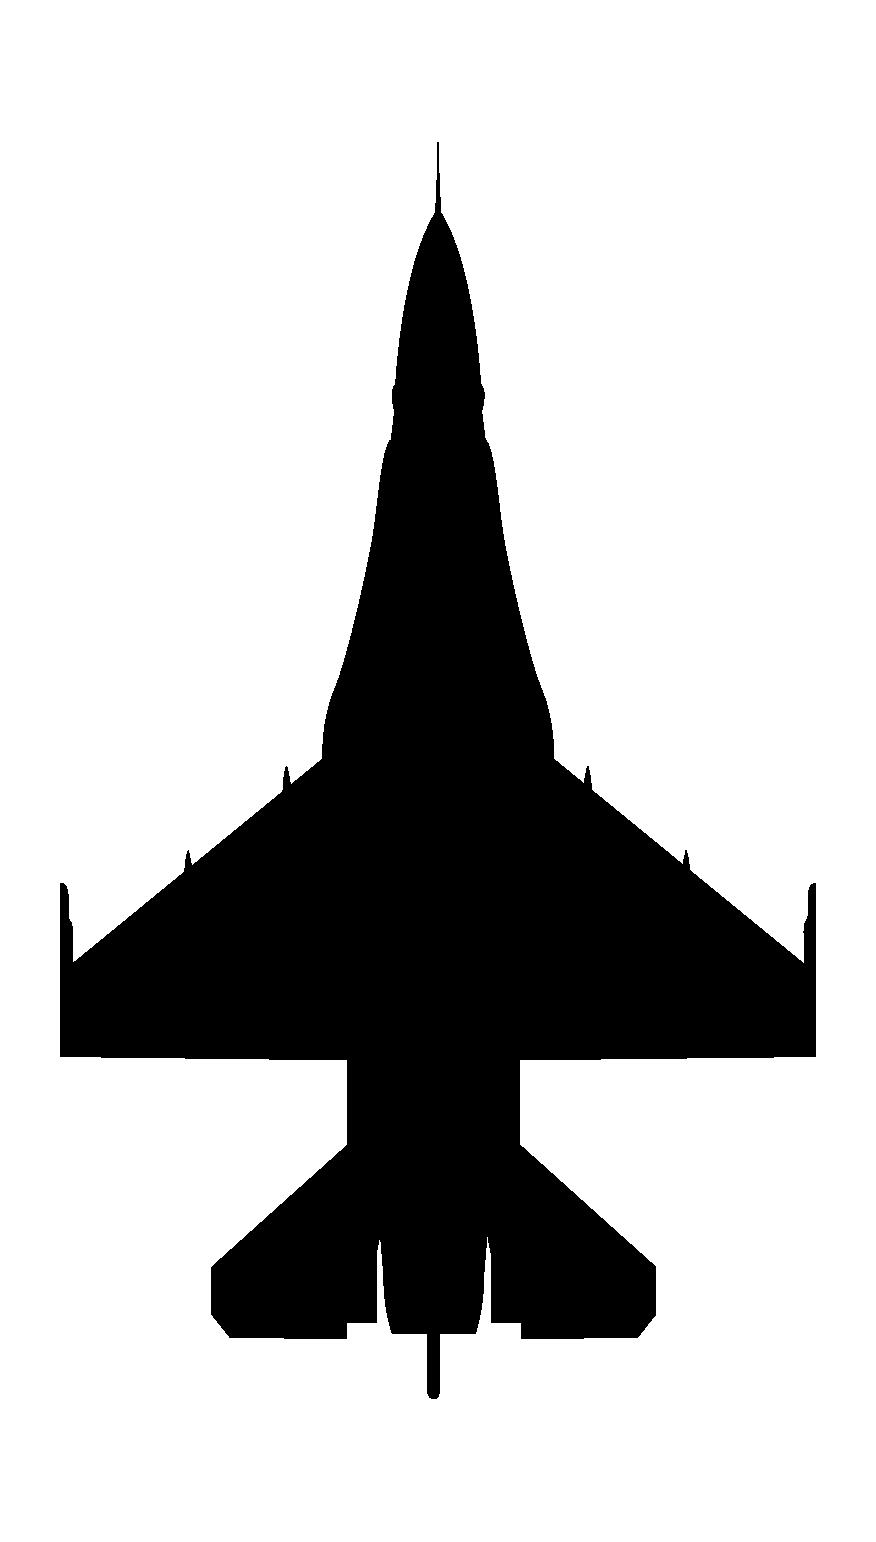
\includegraphics[
                    angle=180,
                    width=7.5mm,
            ]{diagrams/aircraft/silhouette_f16_top.pdf}};

    \end{tikzpicture}
    \caption{Work in progress timeline illustration}
}
\begin{center}
    \vspace{\textheight/4}
    \Large\titlefont\textbf{COMING SOON}
\end{center}

\marginfigrestore